\documentclass{scrartcl}

\usepackage[hidelinks]{hyperref}
\usepackage[none]{hyphenat}
\usepackage{setspace}
%\doublespace Plz no, I need to proofread this

\usepackage{graphicx}
\usepackage{float}
\graphicspath{{images/}}

\newcommand{\source}[1]{\caption*{Source: {#1}} }
% Above code sourced from Xavi, Stack Overflow, https://tex.stackexchange.com/questions/95029/add-source-to-figure-caption @ 20/03/2018

\title{What C++ architecture could best support Quality-of-Experience-oriented map streaming in a multiplayer building game?}
\subtitle{COMP130 - Computing Architecture}
\date{\today}
\author{1707981}

\begin{document}
\maketitle
\pagenumbering{arabic}

\begin{abstract}
Low broadband speeds across the world could hinder the advancement of multiplayer gaming, particularly for traffic-hungry projects such as MMOs or building games. From a creative standpoint, player experience is decidedly the most important factor in a game's design. When downloading the game environment, low bandwidth increases download speeds and temporarily strips players of their autonomy, causing frustration. To aid this, Quality-of-Experience (QoE) techniques are proposed to mitigate the negative effects of limited bandwidth on the player experience, in a way that could be adapted to existing games with minimal difficulty.
\end{abstract}

\section{Introduction}
The games market is continuing to grow at an immense rate, especially in developing countries. In East Asia, a growth of nearly 15\% over the last year has been observed, as shown in Fig. \ref{fig:market}.

\begin{figure}[H]
	\centering
	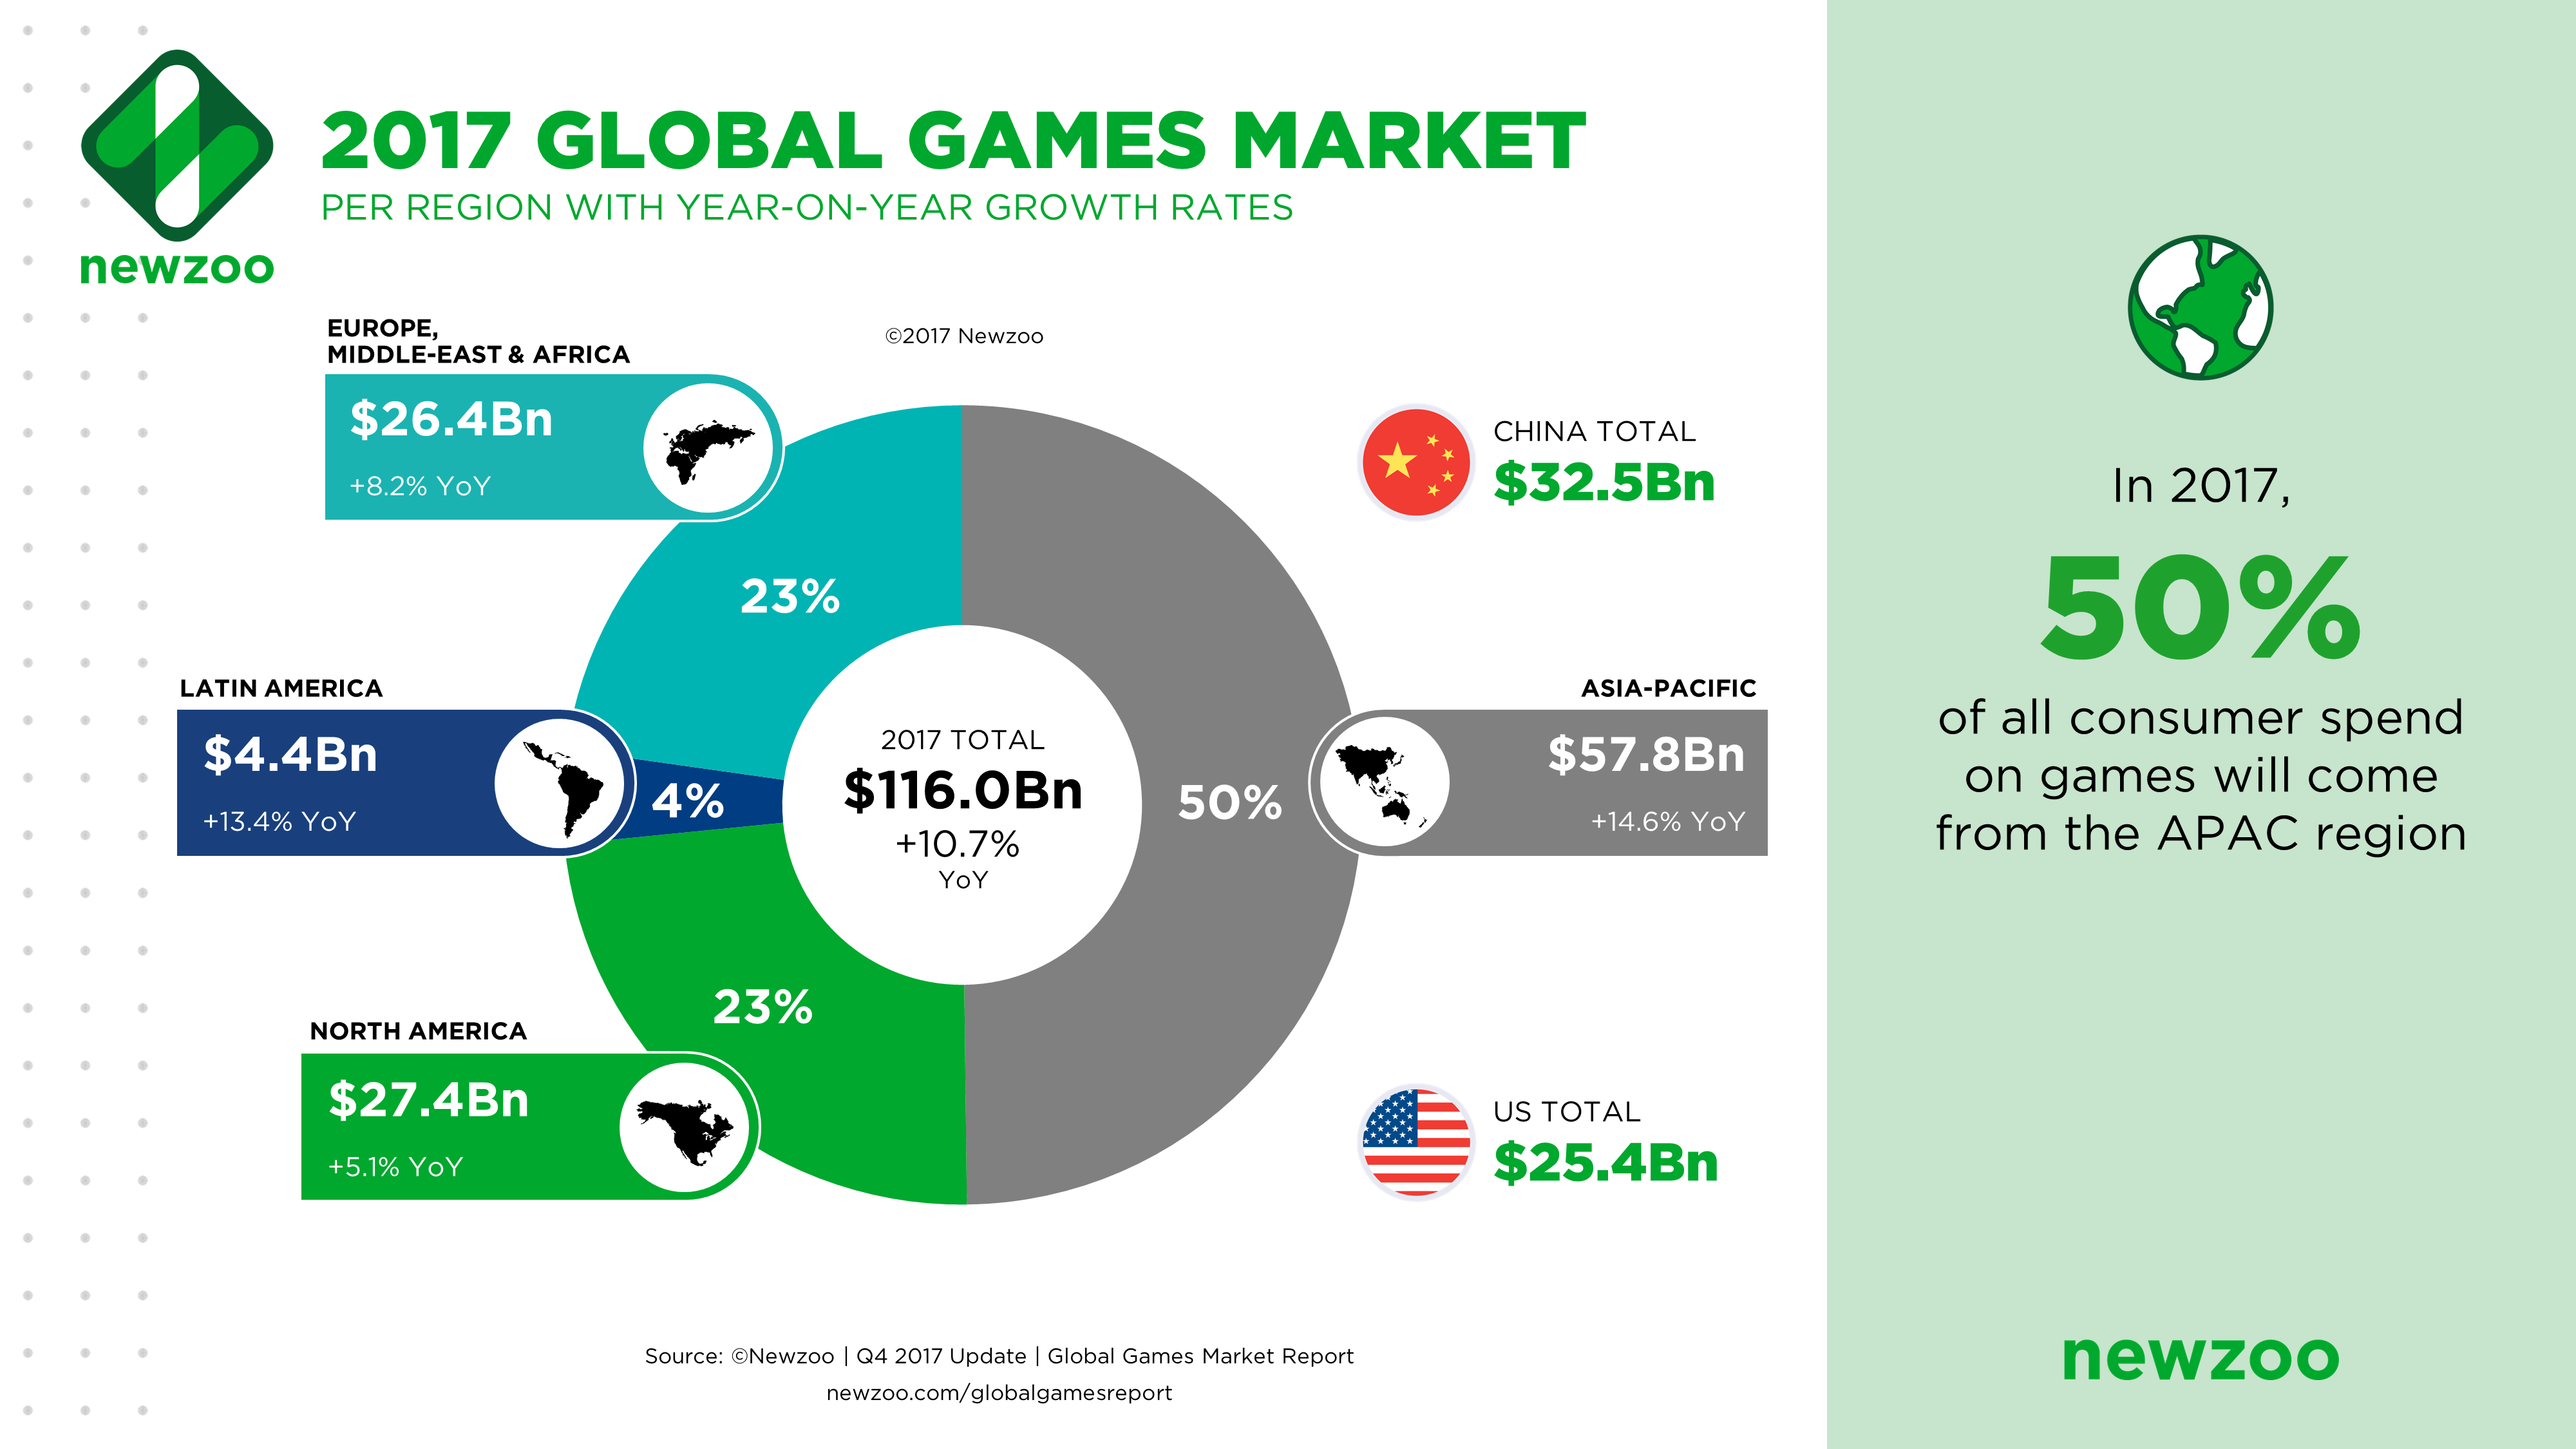
\includegraphics[width=0.75\linewidth]{Newzoo_2017_Global_Games_Market.png}
	\caption{The games market in 2017, according to NewZoo (Source: \cite{globalmarketpic})}
	\label{fig:market}
\end{figure}

This presents profitable opportunities for game developers to expand into new territories. However, a lag in technological advancement, particularly broadband, raises reasonable concerns of whether they can fully exploit these opportunities. The potential of games where players can build the map, such as the extremely popular (as suggested by Google Trends \cite{minecraftnite}) Minecraft and Fortnite, may be hindered by a lack of bandwidth necessary to download player-built resources at an acceptable speed. A slow download of map resources may frustrate players by rendering them unable to access areas of the game in a timely manner.

This study aims to discover the extent of this problem, followed by proposals of architectural methods to implement systems that could mitigate the negative effects of an unreliable networking environment on the player experience. These can be described as QoE (Quality-of-Experience) improvements where the bandwidth is not improved, but instead coordinated toward where the player needs it most. The programming language in question is C++, while the hypothetical game assumed a 3D environment wherein the player can manipulate the terrain and build meshes. The goal is to propose a reasonable set of design patterns to be used for QoE-oriented map streaming in a large-scale game, and how they could be applied to an existing game engine.

This analysis will take place over the following steps:

\begin{itemize}
\item Exploration into the games market and its broadband speeds,
\item A brief introduction to player experience as a separate concept to content quality, to gain an understanding of what should be prioritised,
\item A priority list of assets and features of immediate interest to the player, and
\item A proposed technical outline of a system that could facilitate level streaming with priority on player experience
\end{itemize}

\section{The Big, Slow Market}
China is the most profitable games market as of 2017 \cite{chinamarket}. Furthermore, according to SteamSpy in March 2018, 8 of the 10 most popular Steam games in China were partly or fully multiplayer \cite{steamchina}. This suggests China is a valuable target for online games. However, compared to most developed countries, China's Internet speeds lag behind (figuratively speaking), at an average of 7.6Mbps \cite{webspeeds}.

Similarly, another country notorious for its online gaming community is Brazil. According to SteamSpy, 9 of the top 10 games had a multiplayer component, with 8 boasting primarily multiplayer gameplay \cite{steambrazil}. Brazil's Internet speed averaged about the same--6.8Mbps--in 2017 \cite{webspeeds} (an ironic failing for the world's fifth top source of DDoS attacks in early 2017 \cite{websecurity}).

Speeds in the UK and US meanwhile average at over twice as much, 16.9Mbps and 18.7Mbps respectively. While this study was originally expecting a bigger discrepancy, it could surmise that the map streaming engines of large-scale player-built online games will require optimisation to compensate the lack of data bandwidth compared to, for example, disk speeds. In the Sony PS4's case, streaming speed from the disc maxes out at 27MB/s (at a 1x speed of 36Mbps \cite{bluray} multiplied by 6 \cite{ps4specs})--a significantly higher rate than Brazil's average Internet speed of 6.8Mbps, or 0.85 MB/s. This is only 3\% of the typical disc data rate.

There is a lack of definitive research on the impact of low broadband speed in map streaming. A point of reference or scale in terms of user experience is therefore lacking, making the actual negative impacts of low bandwidth relatively uncertain. Until this is further understood, this essay will create the system around scalable broadband speed, aiming to guarantee an acceptably 'fun' quality even in extremely slow network conditions. However, the definition of 'fun' may be at odds with the industry's tendency to create games that are bigger, more detailed, and overall more data-heavy as they evolve \cite{graphicsvsexperience}. This prompts an exploration into what is 'fun', in a term more aptly described as quality of experience.

\section{Quality of player experience} \label{player}
Video streaming is a heavily researched area; perhaps more than games, owing to significant dedicated R\&D toward streaming services such as the Amazon FireTV \cite{amazonresearch}. Yet considering the link between video quality and quality of gameplay aesthetic--including pixel resolution, lag spike rate, and frame rate--the basic principles and goals could perhaps apply to games as well.

In the context of video, it has been documented \cite{qoelargestudy} that user enjoyment is greater in a scenario of low-detail, constant frame streaming, than one of higher-detail, inconsistent frame streaming. In other words, the user is not interested in the rate of high-detailed data, but in enjoying a smoother experience.

In the context of games, this smooth experience is also shown to be necessary to retain game players. Studies have noted latency \cite{qossensitivity} \cite{lagragequits}, jitter and packet loss \cite{lagragequits} to all have negative impacts, sometimes leading to quitting altogether. While this is not widely studied in building games--but FPSes and MMOs--games such as the recent and highly popular \cite{topgames} Fortnite, which features both building elements and shooting gameplay, demonstrates that the two are not necessarily mutually exclusive.

Another study \cite{graphicsvsexperience} noted the importance of animations in a game. Similarly, this centres around the concept of motion, and as above, suggests that graphical detail is of smaller importance than the player's ability to gain immediate feedback. This is supported at a base psychological level by R. Ryan and E. Deci's reputable research on human motivation \cite{motivation} (noteworthy in that they have disproportionately few people to cite, other than themselves, throughout their entire paper), which notes a human desire to explore, apply their skills, and learn from the feedback.

These findings place high importance on the motion, control, and abilities of the player rather than visual fidelity of the background. In map streaming, this translates to the importance of giving the player base landscapesto move within and toward. This places the level mesh, and perhaps interactive objects (noting the need for motion), above textures and sounds in the priority list.

\section{Quality of experience -- Priorities}
To maximise player experience, a preliminary priority list is thus proposed:

\begin{itemize}
	\item Player movement
	\item Player avatar
	\item Untextured level geometry (nearby)
	\item Interactive objects
	\item Player animations
	\item Object animations
	\item Untextured level geometry (distant, low-detail)
	\item Textures
	\item Additional resources
\end{itemize}

However, this is not an exact science. For example, level textures may come in a low-quality form before their final form. This would show evidence of loading progress to the player. While it could be argued as invasive, a player would likely deem this more favourable than--for example--a loading screen, as observed in software studies \cite{loadingscreens}. Furthermore, level textures might not necessarily be streamed, unless the players should be able to draw their own.

As an additional note, the specifics of animation, player model, object and texture streaming are beyond the scope of this essay, but are noted above for the reader's interest.

\section{Proposal}
The proposed system base, designed to prioritise the player experience, is illustrated below as two components, the client component and server component. These represent the game and the persistent online server, respectively.

\subsection{Server system}
\begin{figure}[H]
	\centering
	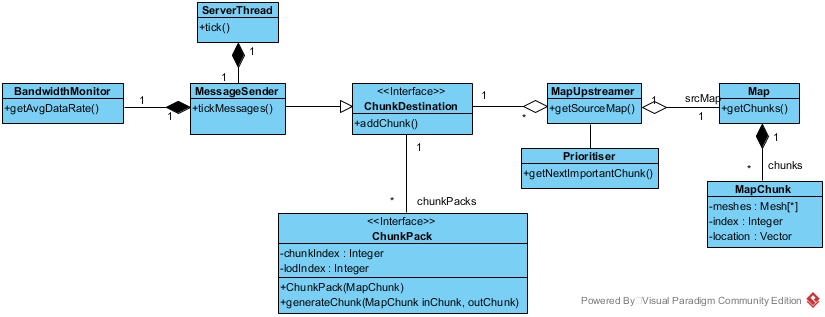
\includegraphics[width=0.7\linewidth]{Server_Side_Streamer.png}
	\caption{Partial class diagram illustrating the potential map streaming server},
	\label{fig:serversystem}
\end{figure}

The proposed system would comprise the following key classes:

\begin{itemize}
\item \textbf{Map}: The base map class. This is shared between the client and server. By partitioning the map into several \textbf{MapChunks}, separate pieces of it can be downloaded at a time, allowing the player to roam incomplete areas in short notice.
\item \textbf{MapChunk}: A portion of the map, with an index identifying the specific area of the level, and mesh information. The shape of a level chunk may vary across games, though in a building game, a uniform shape could be chosen such that there is consistency in the efficiency of building in one place over another. However, different games may use different strategies. For example, Sunset Overdrive (Insomniac Games, 2014) used hexagonal chunks by design and radial chunks in practice. This was optimised for the player's freedom of movement. However, an earlier game by the same company, Fuse (Insomniac Games, 2013), used rectangular chunks. This was optimised for linear hall-based gameplay \cite{overdrivegdc}.
\item \textbf{ChunkDestination}: A collection of \textbf{ChunkPacks} that may be implemented in multiple ways. In this case, it is connected to \textbf{MessageSender} for immediate transmission. In more advanced cases, it could also, at a later stage, be implemented on the client machine as a map storage manager, which could cache map data on a local machine for later use.
\item \textbf{MapUpstreamer}: The MapUpstreamer is effectively a \textit{Mediator} (described as a class that manages the collaboration between objects \cite{designpatterns}) technically owned by neither Map nor ChunkDestination. This method was chosen so that MapUpstreamer could, if necessary, operate independently in parallel to the other tasks. An observer pattern could reasonably be used, but this typically means synchronising the data on an immediate basis \cite{designpatterns}, something which is not necessary for the time-sensitive task of prioritising the data flow.
\item \textbf{BandwidthMonitor}: To achieve data rate consistency as likely desired by players (see Section \ref{player}), this class monitors bandwidth over time and adjusts the data rate to the most consistent possible. The specifics of this system, better described as bandwidth-smoothing, are beyond the scope of this essay. A broad comparison of bandwidth-smoothing techniques as illustrated by W. Feng and J. Rexford is recommended for further reading \cite{bandwidthsmoothing}.
\item \textbf{ChunkPack}: This interface stores components of map data in various possible class-specific ways, and provides the function \textit{generateChunk} such that it can inject itself into the Map. An example of a child class--\textbf{ChunkPack\_Delta}--is demonstrated in Fig. \ref{fig:clientsystem}.
\end{itemize}

\subsection{Client system}
\begin{figure}[H]
	\centering
	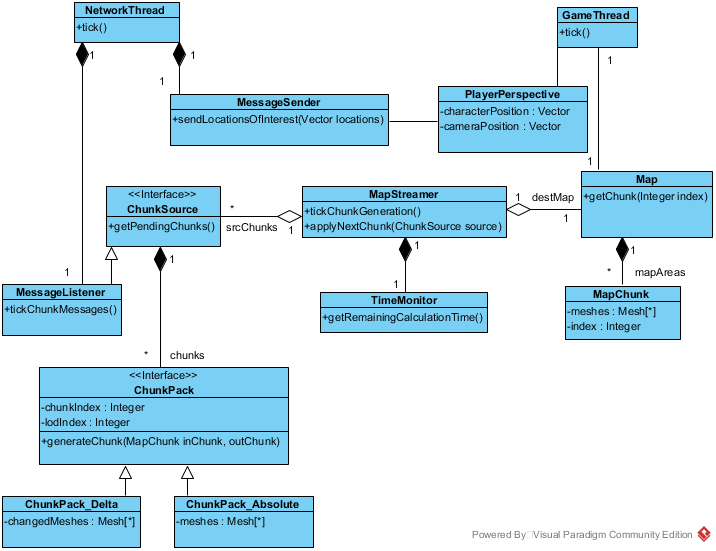
\includegraphics[width=0.7\linewidth]{Client_Side_Streamer.png}
	\caption{Partial class diagram illustrating the potential map streaming client},
	\label{fig:clientsystem}
\end{figure}

To support the independence of the background download process, which focuses on delivering data in a time-sensitive manner, this process is divided into two concurrent threads. This system comprises the following key classes, some of which are shared with the Server system:

\begin{itemize}
\item \textbf{MapStreamer}: Responsible for collecting \textbf{ChunkPack}s and transferring them to the physical \textbf{Map} when it deems appropriate. This is another example of a Mediator. It relies on \textbf{TimeMonitor} to deliver the chunks smoothly.
\item \textbf{TimeMonitor}: To ensure a smooth experience, this determines the amount of processing time to dedicate to chunk generation. This will be dependent on the game's other systems, and there are many factors to consider--such as used CPU time, network speed, the time it takes to generate an average chunk--to optimise this delivery time.
\item \textbf{PlayerPerspective}: Responsible for informing the server where the player is in the map, so that the server can prioritise chunk delivery.
\item \textbf{ChunkData\_Absolute}: Contains a complete map chunk at a certain level of detail.
\item \textbf{ChunkData\_Delta}: Contains a map chunk in terms of changes that have occurred since an earlier version. This will be useful for player building events; for example, when a player constructs a wall. Contrast with rebuilding a mesh from scratch, this may return meshes that have been added or removed.
\end{itemize}

The class diagram above depicts the client end of the map streaming game component. Flow takes place in the following fashion:

\begin{figure}[H]
	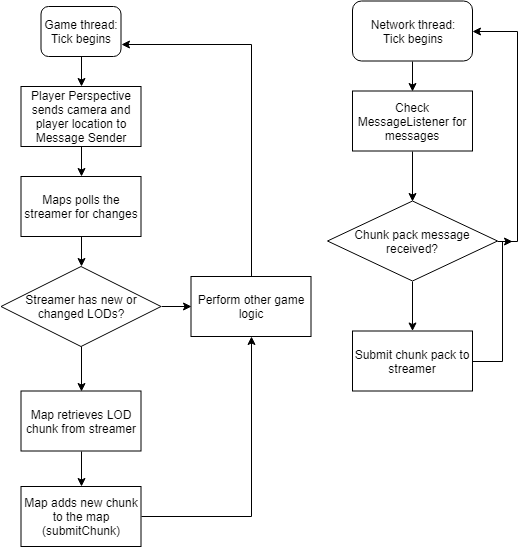
\includegraphics[width=0.7\linewidth]{Basic_Flowchart.png}
	\caption{Process flow of the two threads in parallel}
	\label{fig:simpleflow}
\end{figure}

In this example, the client begins by sending the player and camera location as soon as possible. Sometimes these two variables may be different: it is important that both areas are prepared for the player's viewing. The server is assumed to prioritise the level chunk geometry from closest to furthest.

\section{Conclusion}
A system architecture focusing on delivering data to the player in a consistent \cite{qoelargestudy} \cite{lagragequits}, immediately interactive \cite{motivation}, and smooth \cite{graphicsvsexperience} \cite{lagragequits} way is proposed to optimise the player experience. While the environment was states to be C++, it is likely that this architecture could be applied to most modern object-oriented languages.

There is much room for further research and expansion, including but not limited to compression, variable chunk scaling, texture streaming, gameplay element streaming and sound streaming techniques. Furthermore, lack of research on the impact of bandwidth on building games leaves the true fidelity and efficiency requirements of this system to be quite undefined. This may be prompted by the development of more games of this type, which could facilitate further research into the connectivity requirements globally. Noting the popularity of Fortnite today, which now matches Minecraft \cite{minecraftnite}, this could be expected to happen in the near future.

\bibliography{references} 
\bibliographystyle{ieeetr}

\end{document}